\title{Image processing with graphs}

This is one of the best books in image processing:

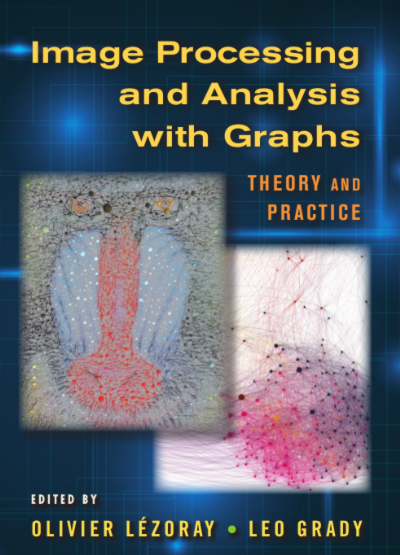
\includegraphics{i/graphcover.png}

You should buy several copies, for yourself, your friends and your family;
and ask your lab to buy several copies for the library.  Or even better,
since the editor (whose name I have trimmed from the cover image) is a
notorious bully, instead of buying it, download a copy from libgen and send
the money directly to the authors.

The book is a collection of independent self-contained chapters written by
different authors, all of them famous people from the french school of image
processing.

The only critique of this book that I can conceive is that the ``practice''
part of the title is not really fullfilled.  There is not a single line of
real computer code displayed in the book.  But giving the codes for the
hundreds of experiments of a 500 page book is probably too much to ask.  The
goal of this document is to provide such a code for a small part of the book.

My favourite chapters are 6 and 7:

{\bf 6. A short tour of mathematical morphology on edge and vertex weighted
graphs}, {\it Laurent Najman and Fernand Meyer}

{\bf 7. Partial difference quations on graphs for local and nonlocal image
processing}, {\it Abrerrahim Elmoataz, Olivier Lézoray, Vinh-Thong Ta and
Sébastien Bougleux}.

And these are the chapters whose implementation I detail below.


\section{The basic approach}

The book contains this kind of sentences:

\newcommand{\R}{\mathbf{R}}

\begin{quote}
Let $G=(V,E)$ be a graph and $\mathcal{H}(V)$ be the Hilbert space of
real-valued functions defined on the vertices of~$G$.  The
space~$\mathcal{H}(V)$ is endowed with the usual inner
product~$\left<f,h\right>_{\mathcal{H}(V)}=\sum_{v_i\in V}f(v_i)h(v_i)$,
where~$f,h:V\to\R$.
Similarly, let~$\mathcal{H}(E)$ be the Hilbert space of real-valued functions
defined on the edges of~$G$,~$\ldots$.  Now, consider a linear operator
between Hilbert spaces~$A:\mathcal{H}(V)\to\mathcal{E}(V)$...
\end{quote}

While these sentences are crystal clear and very appealing to an audience of
mathematicians, I have found them to be intimidating when trying to
evangelize people to read the book.  Thus, I ``translate'' them into the
following kind of language, which is~$100\%$ equivalent:

\begin{quote}
Consider a graph with~$n$ vertices and~$m$ edges.  We will use vectors
of length~$n$ and $m$ to represent functions defined over the vertices or
the edges, respectively.  We will also use matrices of size~$m\times n$
to represent linear maps between them~$A:\R^n\to\R^m$.  In octave/matlab:

\begin{verbatim}
n = 100;            # number of vertices in the graph
m = 200;            # number of edges in the graph
x = rand(n,1);      # define a random function over the vertices
A = rand(m,n);      # define a random linear map
y = A * x;          # obtain a function over the edges
\end{verbatim}
\end{quote}

This is easier to interpret thanks to the computer code.  Of course, linear
maps with random coefficients are silly.  We will see more interesting
examples below.


\section{Matrices of a graph}

You would think that to work with graphs on a computer you need some sort of
library for graphs.  Nothing farther from the truth.  What you really need is
a library for doing~\emph{linear algebra}.  In all the examples here we use
octave, but you can translate it easily to python+numpy, which is slightly
more verbose.

In what follows we reserve the letters~$n$ and~$m$ for the following meanings

$n\, =\ \,$ number of vertices in the graph\newline
$m =\ \,$ number of edges in the graph

For the following graph, we have~$n=5$ and $m=6$:

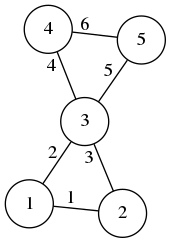
\includegraphics{gggx.png}
%SCRIPT echo 'graph { node [shape=circle]
%SCRIPT 1--2 [label="1"]
%SCRIPT 1--3 [label="2"]
%SCRIPT 2--3 [label="3  "]
%SCRIPT 3--4 [label="4  "]
%SCRIPT 3--5 [label="5"]
%SCRIPT 4--5 [label=" 6 "]
%SCRIPT }' | neato -Tpng > gggx.png

$$
Z = \begin{pmatrix}
1 & 2 \\
1 & 3 \\
2 & 3 \\
3 & 4 \\
3 & 5 \\
4 & 5
\end{pmatrix}_{\small 6\times 2}
A = \begin{pmatrix}
	0 & 1 & 1 & 0 & 0 \\
	1 & 0 & 1 & 0 & 0 \\
	1 & 1 & 0 & 1 & 1 \\
	0 & 0 & 1 & 0 & 1 \\
	0 & 0 & 1 & 1 & 0 \\
\end{pmatrix}_{\small 5\times 5}
B = \begin{pmatrix}
	-1& 1 & 0 & 0 & 0 \\
	-1& 0 & 1 & 0 & 0 \\
	0 &-1 & 1 & 0 & 0 \\
	0 & 0 &-1 & 1 & 0 \\
	0 & 0 &-1 & 0 & 1 \\
	0 & 0 & 0 &-1 & 1 \\
\end{pmatrix}_{\small 6\times 5}
$$

There are {\bf five} basic matrices associated to a graph, for which we will
always use the same letters:

$Z\ \,=\ \,$ adjacency list, of size $m\times 2$,
             list of vertex index pairs \newline
$A\ \,=\ \,$ adjacency matrix, of size $n\times n$,
             logical matrix of joined vertices \newline
$B\ \,=\ \,$ incidence matrix, of size $m\times n$,
             list of input/output vertices of each edge \newline
$C\ \,=\ \,$ centering matrix, of size $m\times n$,
             defined as~$C=\frac{1}{2}|B|$ \newline
$L\ \,=\ \,$ Laplacian matrix, of size $n\times n$,
             defined as~$L=-B'B$

It is very important to understand now the meaning of the matrices~$Z,A,B$.
The matrix~$Z$ is the easiest to type by hand in a computer, but it is not
very useful for doing algebra with it.  All the other matrices are
fundamental linear operators over functions defined on the graph.  Each of
these fives matrices, alone, determines completely the graph (modulo the
numbering of the edges, in the case of~$A$ and~$L$).

The matrices~$A$, $B$ and~$C$ satisfy the identity: $A=2C^TC-B^TB/2$.  This
allows to compute~$A$ from~$B$.  To recover~$B$ from~$A$ we must decide on an
ordering for the edges.

The following octave functions allow to convert between each representation:

%RUN_VERBATIMS octavescript

\begin{verbatim}
function A = graph_adjacency_from_list(Z)
        n = max(Z(:));                        # number of vertices
        U = sparse(Z(:,1), Z(:,2), 1, n, n);  # directed graph
        A = U + U';                           # symmetrization
end
\end{verbatim}

\begin{verbatim}
function B = graph_incidence_from_adjacency(A)
        [i,j] = find(triu(A));                 # find the (i,j) positions
        n = rows(A);                           # number of vertices
        m = rows(i);                           # total number of edges
        B1 = sparse(1:m, i, 1, m, n);          # matrix for destination vertices
        B2 = sparse(1:m, j, 1, m, n);          # matrix for source vertices
        B = B1 - B2;                           # signed incidence matrix
end
\end{verbatim}

\begin{verbatim}
function Z = graph_list_from_adjacency(A)
        [i,j] = find(triu(A));
        Z = [i j];
end
\end{verbatim}

\begin{verbatim}
function A = graph_adjacency_from_incidence(B)
        A = max(-B'*B,0);            # equal to (abs(B'*B) - B'*B) / 2
end
\end{verbatim}

Typically, in the applications, you can often build~$B$ directly so that you
do not really need these functions.  From~$B$, the other matrices are easily
computed if needed by:

 \begin{verbatim}
L = -B'*B;
A = L > 0;
C = abs(B)/2;
\end{verbatim} % spacing necessary to disable execution of this verbatim

The following table summarizes the language that we will use everywhere.

\begin{tabular}{l|l}
	$n$ & number of vertices in the graph \\
	$m$ & number of edges in the graph \\
	$u\in\R^n$ & scalar field~$u$ \\
	$\mathbf{v}\in\R^m$ & scalar field~$\mathbf{v}$ \\
	$B:\R^n\to\R^m$ & gradient \\
	$-B^T:\R^m\to\R^n$ & divergence \\
	$L:\R^n\to\R^n$ & Laplacian \\
	$C:\R^n\to\R^m$ & centering operator (from vertices to edges) \\
	$C^T:\R^m\to\R^n$ & centering operator (from edges to vertices) \\
	$C^TC:\R^n\to\R^n$ & smoothing operator
\end{tabular}

The most important notion is that the matrix~$B$ is called the~{\bf
gradient}.  It is a linear operator that maps scalar fields (vectors of
lenght~$n$) into vector fields (vectors of length~$m$).
This definition is used for an arbitrary graph, but it makes a lot of sense
when the graph is the grid of an image, because in that case the gradient
corresponds exactly to the gradient computed using finite differences.


\section{The graph associated to an image}

The pixels of an image are arranged naturally in the shape of a grid.
Here, for example, you have the grid of a~$4\times 3$ image:

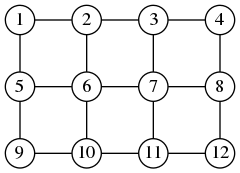
\includegraphics{gridgraph.png}
%SCRIPT echo 'graph {
%SCRIPT node [shape=circle width=0.3 fixedsize=true]
%SCRIPT 1--2--3--4;5--6--7--8;9--10--11--12
%SCRIPT 1--5--9;2--6--10;3--7--11;4--8--12
%SCRIPT 1  [pos="0,100"  ]
%SCRIPT 2  [pos="50,100" ]
%SCRIPT 3  [pos="100,100"]
%SCRIPT 4  [pos="150,100"]
%SCRIPT 5  [pos="0,50"   ]
%SCRIPT 6  [pos="50,50"  ]
%SCRIPT 7  [pos="100,50" ]
%SCRIPT 8  [pos="150,50" ]
%SCRIPT 9  [pos="0,0"    ]
%SCRIPT 10 [pos="50,0"   ]
%SCRIPT 11 [pos="100,0"  ]
%SCRIPT 12 [pos="150,0"  ]
%SCRIPT }' | neato -n -Tpng > gridgraph.png

Here you see that the graph has~$n=12$ vertices and~$m=17$ edges.
In general, for an image of size~$w\times h$, the graph will have~$n=wh$
vertices and~$m=(w-1)h+(h-1)w$ edges.  The matrix~$A$ of such a graph is
build by the following octave code

\begin{verbatim}
function A = grid_adjacency(w, h)                  # build a grid graph WxH
        x = sparse(1:w-1, 2:w, 1, w, w);           # path graph of length W
        y = sparse(1:h-1, 2:h, 1, h, h);           # path graph of length H
        U = kron(y,speye(w)) + kron(speye(h),x);   # kronecker sum
        A = U + U';                                # symmetrization
end
\end{verbatim}

This works because the grid graph is the product graph of two paths, and the
adjacency matrix of a product graph is the Kronecker sum of their matrices.

You can also build the incidence matrix directly, by a similar process

\begin{verbatim}
function B = grid_incidence(w, h)
	x = sparse(1:w-1, 2:w, 1, w, w) - speye(w);  # path of length W
	y = sparse(1:h-1, 2:h, 1, h, h) - speye(h);  # path of length H
	P = kron(speye(h), x);                       # H horizontal W-paths
	Q = kron(y, speye(w));                       # W horizontal H-paths
	B = [ P ; Q ]                                # union of all paths
end
\end{verbatim}

The graph defines just the~\emph{domain} of an image.  We still need the
\emph{data}.  As a sample image, we will use the amazing portrait of Samuel
Beckett by Jane Bown:

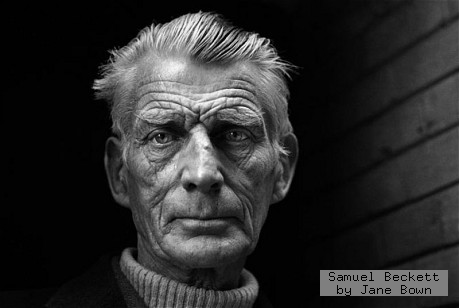
\includegraphics{i/beckett.png}
\verb+beckett.png+

The easiest operator to understand is the Laplacian.  The following octave
code thus reads an image, applies the laplacian operator, and saves the
result.

\begin{verbatim}
x = imread("i/beckett.png");      # load input image
[w, h] = size(x);                 # extract dimensions
x = double(x(:));                 # flatten image data into a vector
A = grid_adjacency(w,h);          # build graph adjacency matrix
L = A - diag(sum(A));             # Laplacian matrix
y = L * x;                        # Laplacian of the original image
z = uint8(reshape(127-2*y,w,h));  # contrast change and reshape
imwrite(z, "beckett-lap.png");    # save output image
\end{verbatim}


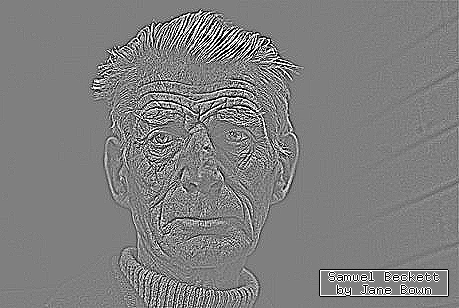
\includegraphics{beckett-lap.png}
\verb+beckett-lap.png+

The typical color coding for looking at a laplacian is such that gray=zero,
white=negative, black=positive.  As expected, the laplacian enhances the
edges and textures while setting the constant regions to zero.

By substracting the laplacian to the image, we ``sharpen'' the original image.

\begin{verbatim}
y = x - L * x;                                        # image minus laplacian
imwrite(reshape(uint8(y),w,h), "beckett-sharp.png");  # save output image
\end{verbatim}
%z = uint8(reshape(y,w,h));          # reshape
%imwrite(z, "beckett-sharp.png");    # save output image

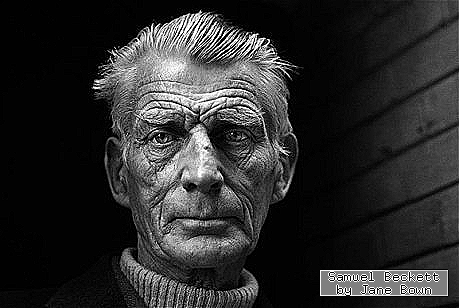
\includegraphics{beckett-sharp.png}
\verb+beckett-sharp.png+

Conversely, we can smooth the image by adding multiples of the laplacian to
it, iteratively.  This amounts to approximation the solution of the heat
equation on the graph:

\begin{verbatim}
S = speye(w*h) + L/4;                                  # smoothing operator
y = S^8 * x;                                           # run 8 smoothing steps
imwrite(reshape(uint8(y),w,h), "beckett-smooth.png");  # save output image
\end{verbatim}
%z = uint8(reshape(y,w,h));          # reshape
%imwrite(z, "beckett-smooth.png");   # save output image

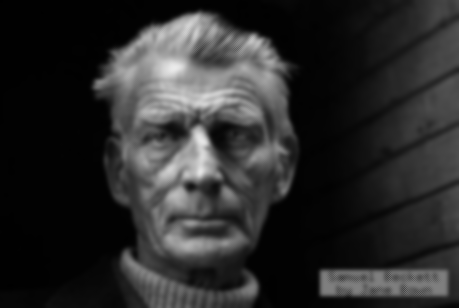
\includegraphics{beckett-smooth.png}
\verb+beckett-smooth.png+

\section{Graph-based mathematical morphology}

The morphological operations of {\bf dilation} and {\bf erosion} are
defined for functions over graphs, as the maximum and minimum value of
neighboring vertices.  The other morphological operations are all defined in
terms of dilation and erosion:

\begin{tabular}{ll}
	$u$ & function defined on the vertices of the graph \\
	$d(u)$ & dilation (max value among neighboring vertices) \\
	$e(u)$ & erosion (min value among neighboring vertices) \\
	$d(e(u))$ & opening \\
	$e(d(u))$ & closing \\
	$d(u) - u$ & inner morphological gradient \\
	$u - e(u)$ & outer morphological gradient \\
	$\frac{1}{2}(d(u) - e(u))$ & centered morphological gradient \\
	$d(u) + e(u) - 2u$ & morphological laplacian \\
	$u - d(u) - e(u)$ & morphological sharpening (image minus laplacian) \\
	$u - d(e(u))$ & top hat (image minus opening) \\
	$e(d(u)) -u$ & bottom hat (closing minus image) \\
\end{tabular}

Due to the inequalities~$e(u)\le u\le d(u)$, we can see that all these
operations (except the laplacian) produce positive images.  The morphological
gradients are also called upwind and downwind derivatives.

Thanks to sparse matrices, the implementation of these operations is very
easy.  The crucial matrix here is the structuring element matrix~$E$, defined
as the adjacency matrix plus the identity

$$
E = A + I_n
$$

The matrices~$A$ and~$E$ define linear operators on the scalar fields of a
graph.  In the particular case when the graph is the grid of an image, they
can be interpreted as shift-invariant filters defined by the following
stencils:

$$
\mathrm{stencil}(A)=
\begin{array}{|c|c|c|}\hline0&1&0\\\hline1&0&1\\\hline0&1&0\\\hline\end{array}
	\qquad
	\qquad
\mathrm{stencil}(E)=
\begin{array}{|c|c|c|}\hline0&1&0\\\hline1&1&1\\\hline0&1&0\\\hline\end{array}
$$

Of course, this interpretation is only valid far from the boundary of the
image domain.  However, bear in mind that the matrix product is a well-defined,
so that the boundary condition is dealt with ``automatically'' by the form of
the graph.

\subsection{Morphology on binary images}


We start with the implementation of mathematical morphology for binary
images, which are also called~\emph{masks}.
This implementation is easier to understand than for the
general gray-scale case.
The {\bf dilation} of a mask~$m$ can be computed simply by multiplying the
mask by powers of the adjacency matrix.  Actually, the {\bf erosion} and the
{\bf median filter} are also computed by the same operation, and they can be
extracted by thresholding the resulting gray-scale image at its minimum,
maximum or central values.

Notice that if you want to apply erosion a certain number of times, you can
multiply by a power of the adjacency matrix!  Morphology is a nonlinear
operation, but the nonlinearity comes from the threshold, not from the
matrix multiplication.

The following code shows the computation of 6 dilations and erosions of the
same mask (a binarization of the Beckett portrait):

\begin{verbatim}
x = imread("i/beckett.png");                             # load image
[w,h] = size(x);                                         # extract dimensions
m = double(x(:) > 66);                                   # flatten and binarize

E = grid_adjacency(w,h) + speye(w*h);                    # structuring element
y = E^6 * m;                                             # apply 6 times
y1 = y > 0;                                              # extract dilation
y2 = !(y < max(y));                                      # extract erosion
y3 = y > max(y)/2;                                       # extract medfilter

f = 255 / max(y);                                        # gray-scale factor
imwrite(logical(reshape(m,w,h)),  "beckett-bin.png");    # save binary mask
imwrite(uint8(reshape(y,w,h)*f),  "beckett-6gray.png");  # save gray-scale
imwrite(logical(reshape(y1,w,h)), "beckett-6dil.png");   # save dilated mask
imwrite(logical(reshape(y2,w,h)), "beckett-6ero.png");   # save eroderd mask
imwrite(logical(reshape(y3,w,h)), "beckett-6med.png");   # save median filter
\end{verbatim}

\begin{gallery}
	\galleryline{beckett-bin.png}
	\galleryline{beckett-6gray.png}
	\galleryline{beckett-6dil.png}
	\galleryline{beckett-6ero.png}
	\galleryline{beckett-6med.png}
\end{gallery}

\subsection{Gray-level morphology}


The implementation of morphology for gray-scale images is a bit more
complicated.  The trick of thresholding the matrix multiplication does not
work anymore, because we are multiplying by a vector that has many different
values (not only zeros and ones).  What we need is a matrix$\times$vector
multiplication that takes the maximum, instead of the sums along each row.
After a few hours of head-scratching, I realized that this is achieved by
multiplying the matrix~$E$ by the diagonal matrix defined by the vector~$x$
(which results in a sparse matrix) and then taking the maximum along rows of
the resulting matrix.  The code is simple, but maybe not evident:

\begin{verbatim}
function y = dilation(E, x)
        y = full(max(diag(x)*E))';    # maximum value along sparse rows
end
\end{verbatim}

Notice that this only works for positive-valued images (otherwise the "max"
is perturbed by the zeros in the sparse matrix, which are not ignored).  If
we want to compute the minimum, this technique does not work because the
minimum on a sparse matrix is always zero!  Yet, we can ``cheat'' and
implement the erosion by computing the dilation of an image in the negative:

\begin{verbatim}
function y = erosion(E, x)
        m = 1 + max(x);
        t = m - x;
        y = m - dilation(E, t);
end
\end{verbatim}

And finally, the implementation of all the morphological operations consists
simply in copying the table above:

\begin{verbatim}
function y = opening(E,x)      y = dilation(E,erosion(E,x));              end
function y = closing(E,x)      y = erosion(E,dilation(E,x));              end
function y = egradient(E,x)    y = x - erosion(E,x);                      end
function y = igradient(E,x)    y = dilation(E,x) - x;                     end
function y = cgradient(E,x)    y = (dilation(E,x) - erosion(E,x)) / 2;    end
function y = mlaplacian(E,x)   y = dilation(E,x) + erosion(E,x) - 2*x;    end
function y = msharpen(E,x)     y = x - mlaplacian(E,x);                   end
function y = tophat(E,x)       y = x - opening(E,x);                      end
function y = bothat(E,x)       y = closing(E,x) - x;                      end
\end{verbatim}

The following code tests all these operations:

\begin{verbatim}
x = imread("i/beckett.png");
[w,h] = size(x);
x = double(x(:));
A = grid_adjacency(w,h);
E = A + speye(w*h);            # structuring element

imwrite(uint8(reshape( dilation(E,x)         ,w,h)), "beckett-dil.png");
imwrite(uint8(reshape( erosion(E,x)          ,w,h)), "beckett-ero.png");
imwrite(uint8(reshape( opening(E,x)          ,w,h)), "beckett-ope.png");
imwrite(uint8(reshape( closing(E,x)          ,w,h)), "beckett-clo.png");
imwrite(uint8(reshape( 2*igradient(E,x)      ,w,h)), "beckett-igrad.png");
imwrite(uint8(reshape( 2*egradient(E,x)      ,w,h)), "beckett-egrad.png");
imwrite(uint8(reshape( 2*cgradient(E,x)      ,w,h)), "beckett-cgrad.png");
imwrite(uint8(reshape( 127-2*mlaplacian(E,x) ,w,h)), "beckett-mlap.png");
imwrite(uint8(reshape( msharpen(E,x)         ,w,h)), "beckett-msharp.png");
imwrite(uint8(reshape( 6*tophat(E,x)         ,w,h)), "beckett-top.png");
imwrite(uint8(reshape( 255-6*bothat(E,x)     ,w,h)), "beckett-bot.png");
\end{verbatim}

\begin{gallery}
	\galleryline{beckett-dil.png}
	\galleryline{beckett-ero.png}
	\galleryline{beckett-ope.png}
	\galleryline{beckett-clo.png}
	\galleryline{beckett-igrad.png}
	\galleryline{beckett-egrad.png}
	\galleryline{beckett-cgrad.png}
	\galleryline{beckett-mlap.png}
	\galleryline{beckett-msharp.png}
	\galleryline{beckett-top.png}
	\galleryline{beckett-bot.png}
\end{gallery}

It is an interesting exercise to look at these images and try to describe the
changes verbally.  For example: {\bf dilation} enlarges the light objects,
while {\bf erosion} enlarges the dark ones.  The {\bf opening} removes the
small bright spots and ridges, while {\bf closing} removes the small dark
spots and valleys.  All the three {\bf gradients} look like the euclidean
norm of the linear gradient.  The {\bf inner} and {\bf outer} gradients are
very sharp, but are not centered, each one biased towards the dark or the
light side of the discontinuities.  The {\bf centered} gradient is the
average of the two, which is centered but less sharp.  The {\bf morphological
laplacian} is the difference of the inner and outer gradients; it looks
almost exactly like the linear laplacian despite being a combination of
nonlinear operations.  The {\bf morphological sharpening} is similar to the
linear one, based on the reverse heat equation.  The {\bf top-hat} keeps only
the britght spots and ridges (those that were removed by the opening), and
set to zero the rest of the image.  The {\bf bottom-hat} keeps only the dark
spots and valleys (those that were removed by the closing), and sets to zero
the rest of the image; thus the bottom-hat produces an image in the negative,
that must be negated to visualize it correctly.


\section{Linear PDE on graphs}

(section in preparation)

\subsection{Linear second-order equations}

\subsection{Linear first-order equations}


% vim:set tw=77 filetype=tex spell spelllang=en:
